\appendix{Apêndice A: }
\label{apen:a}


\section{Transformação de planilha para banco de dados}
\label{apen:a1}

\begin{figure}[htb]
	\centering					
	{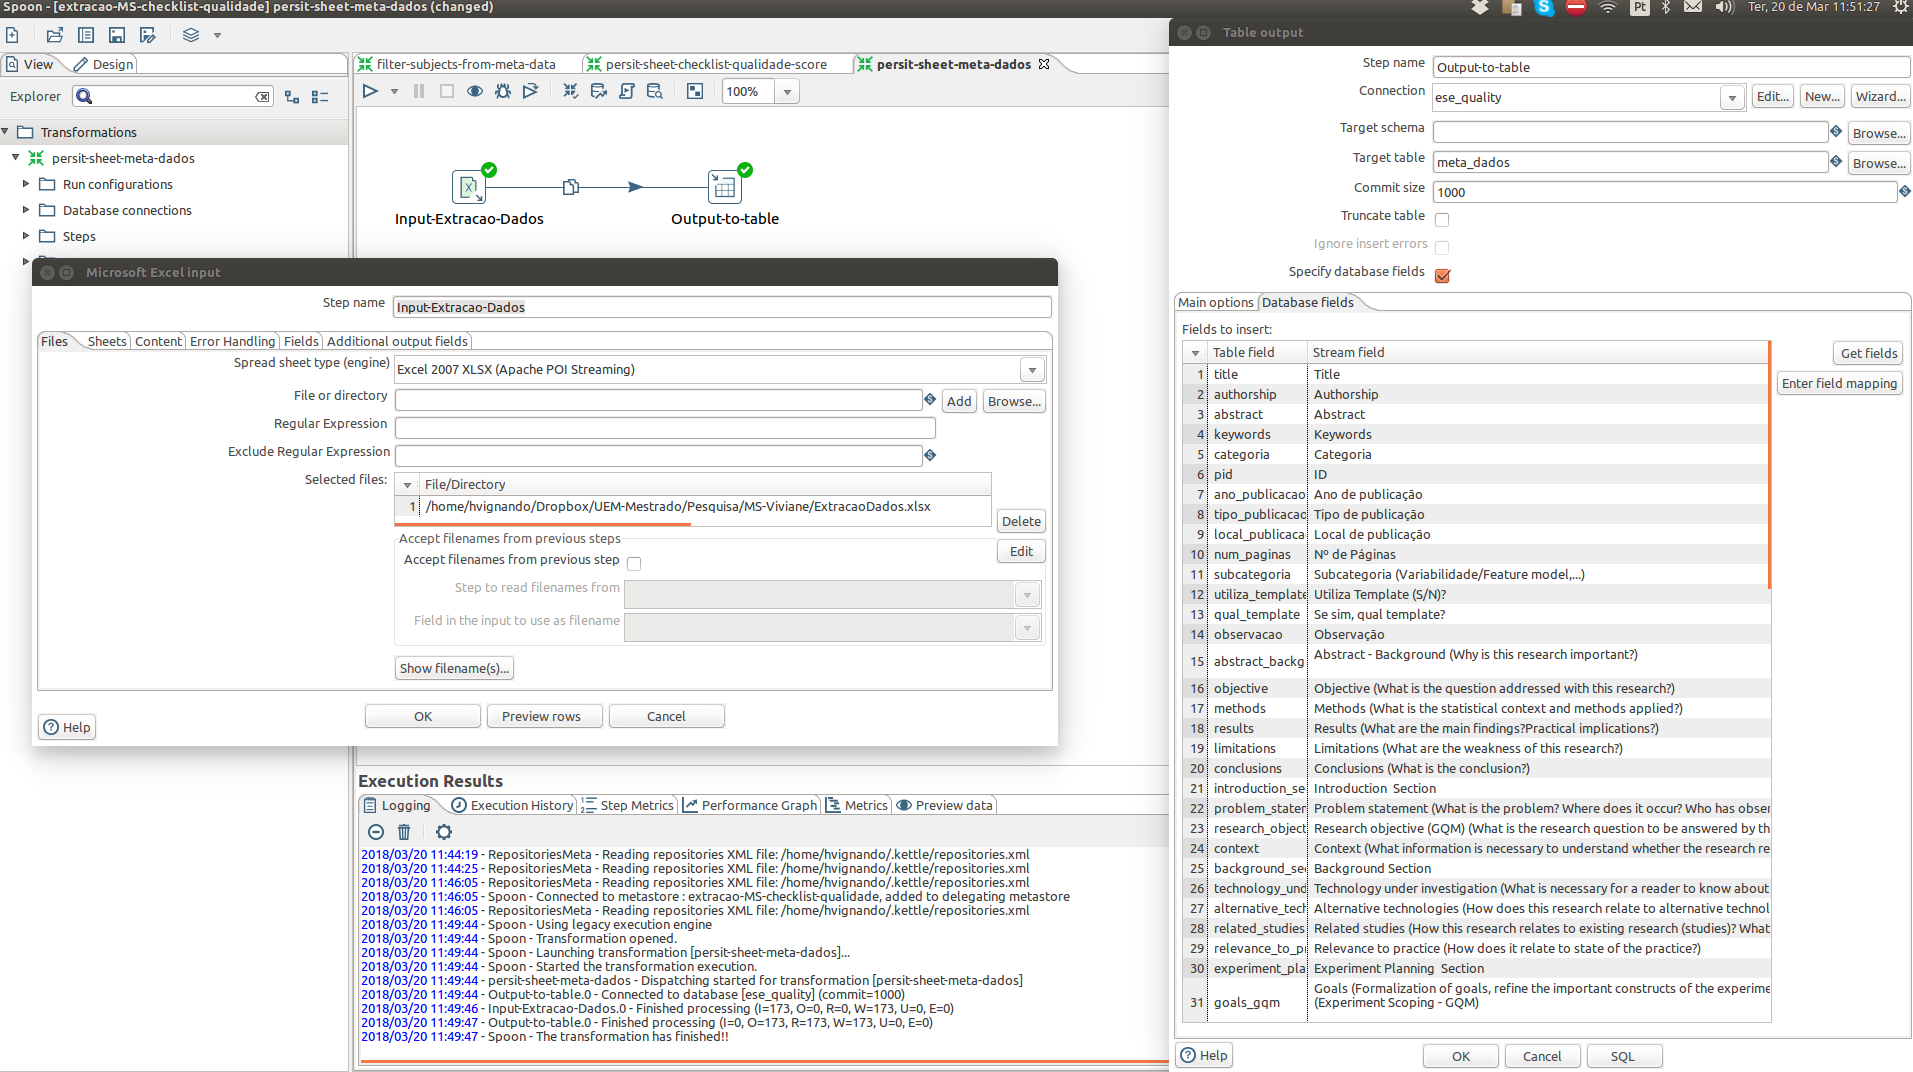
\includegraphics[scale=.23]{etl_extracao_meta_dados.png}}
	
	\caption{Transformação de planilha para uma tabela no banco de dados}
	\label{fig:etl-meta-dados}
\end{figure}

O \textit{Script} \textit{sql} abaixo apresenta a estrutura da tabela para persistência dos dados.
\begin{scriptsize}
	\begin{verbatim}
	CREATE TABLE `meta_dados` (
	`id` int(11) NOT NULL AUTO_INCREMENT,
	`pid` text,
	`title` text,
	`authorship` text,
	`ano_publicacao` double DEFAULT NULL,
	`tipo_publicacao` text,
	`local_publicacao` text,
	`abstract` text,
	`keywords` text,
	`num_paginas` double DEFAULT NULL,
	`categoria` text,
	`subcategoria` text,
	`utiliza_template` text,
	`qual_template` text,
	`observacao` text,
	`abstract_background` text,
	`objective` text,
	`methods` text,
	`results` text,
	`limitations` text,
	`conclusions` text,
	`introduction_section` text,
	`problem_statement` text,
	`research_objective_gqm` text,
	`context` text,
	`background_section` text,
	`technology_under_investigation` text,
	`alternative_technologies` text,
	`related_studies` text,
	`relevance_to_practice` text,
	`experiment_planning_section` text,
	`goals_gqm` text,
	`context_selection` text,
	`experimental_units` text,
	`experimental_material` text,
	`tasks` text,
	`hypotheses` text,
	`parameters` text,
	`variables` text,
	`experiment` text,
	`procedure` text,
	`analysis_procedure` text,
	`execution_section` text,
	`preparation` text,
	`execution` text,
	`deviations_the_plan` text,
	`analysis_section` text,
	`descriptive_statistics` text,
	`dataset_preparation` text,
	`hypothesis_testing` text,
	`discussion_section` text,
	`evaluation_results_implications` text,
	`threats_validity` text,
	`inferences` text,
	`lessons_learned` text,
	`conclusions_futurework_section` text,
	`summary` text,
	`impact` text,
	`future_work` text,
	`acknowledgements_section` text,
	`references_section` text,
	`appendices_section` text,
	`possui_analise_qualitativa` text,
	`qual_analise_qualitativa_realizada` text,
	`utilizou_abordagem_avaliarexperimento` text,
	`conclusao_baseado_pvalue` text,
	`pacote_experimental_informado` text,
	`como_participantes_foram_selecionados` text,
	`is_quasi-experimento` text,
	`has_projeto_piloto` text,
	`original_ou_replicado` text,
	`tipo_experimento` text,
	`colaboracao_parceiraempresa_instituicao` text,
	`has_meta-analise` text,
	`tipo_projeto_experimental` text,
	`tipo_artefato_lps_utilizado` text,
	`lps_real_ou_academica` text,
	`nome_lps` text,
	`has_link_lps` text,
	`ameacas_validade_especificas_lps` text,
	`has_modelo_qualidade_lps` text,
	`has_fatores_qualidade_exp_ou_quasi-exp_lps` text,
	PRIMARY KEY (`id`)
	) ENGINE=InnoDB AUTO_INCREMENT=347 DEFAULT CHARSET=latin1;
	\end{verbatim}
\end{scriptsize}

%\section{SQL para filtrar experimentos que usam subjects}
%\label{apen:a2}
%
%Nesta etapa do desenvolvimento foi construída uma \textit{query} para filtrar os experimentos que usam pessoas como participantes do experimento, essa \textit{query} pode ser vista abaixo. Os experimentos resultantes desta consulta servirá como base para realização da inferência da ontologia.
%
%\begin{scriptsize}
%	
%	\begin{verbatim}
%	SELECT * FROM meta_dados
%	WHERE 1=1
%	and LOWER(abstract) like '%subject%' 
%		or LOWER(title) like '%subject%'
%		or LOWER(keywords) like '%subject%'
%		or LOWER(conclusions) like '%subject%'
%		or LOWER(abstract_background) like '%subject%'
%		or LOWER(experimental_units) like '%subject%'
%		or LOWER(experimental_material) like '%subject%'
%		or LOWER(descriptive_statistics) like '%subject%'
%		or LOWER(tasks) like '%subject%'
%		or LOWER(`procedure`) like '%subject%'
%		or LOWER(execution) like '%subject%'
%		or LOWER(objective) like '%subject%'
%		or LOWER(dataset_preparation) like '%subject%'
%		or LOWER(evaluation_results_implications) like '%subject%'
%		or LOWER(threats_validity) like '%subject%'
%		or LOWER(summary) like '%subject%'
%		or LOWER(`context`) like '%subject%'
%		or LOWER(qual_analise_qualitativa_realizada) like '%subject%'
%		or LOWER(preparation) like '%subject%'
%		or LOWER(research_objective_gqm) like '%subject%'
%		or LOWER(ameacas_validade_especificas_lps) like '%subject%'
%		or LOWER(results) like '%subject%'
%		or LOWER(inferences) like '%subject%'
%		or LOWER(hypotheses) like '%subject%'
%		or LOWER(experiment_planning_section) like '%subject%'
%		or LOWER(como_participantes_foram_selecionados) like '%subject%'
%		or LOWER(problem_statement) like '%subject%'
%		or LOWER(acknowledgements_section) like '%subject%'
%		or LOWER(colaboracao_parceiraempresa_instituicao) like '%subject%'
%		or LOWER(lessons_learned) like '%subject%'
%		or LOWER(problem_statement) like '%subject%'
%	;
%	\end{verbatim}
%% \end{scriptsize}

\section{SQL para listar diretrizes comuns}
\label{apen:a2}

O \textit{Script} \textit{sql} abaixo apresenta as sete \textit{querys} para levantar as informações iniciais de \textbf{ABox}
\begin{scriptsize}
	\begin{verbatim}
	SELECT distinct qual_template
	FROM ese_quality.meta_dados
	where utiliza_template = 'S';
	
	SELECT distinct qual_analise_qualitativa_realizada
	FROM ese_quality.meta_dados
	where possui_analise_qualitativa = 'S';
	
	SELECT distinct categoria
	FROM ese_quality.meta_dados;
	
	SELECT distinct subcategoria
	FROM ese_quality.meta_dados;
	
	SELECT distinct como_participantes_foram_selecionados
	FROM ese_quality.meta_dados;
	
	SELECT distinct tipo_projeto_experimental
	FROM ese_quality.meta_dados;
	
	SELECT distinct tipo_artefato_lps_utilizado
	FROM ese_quality.meta_dados;
	\end{verbatim}
\end{scriptsize}


\section{Grafo inicial de diretrizes para base ontológica de qualidade de experimentos em LPS}
\label{apen:a3}

\begin{figure}[h]
	\centering					
	{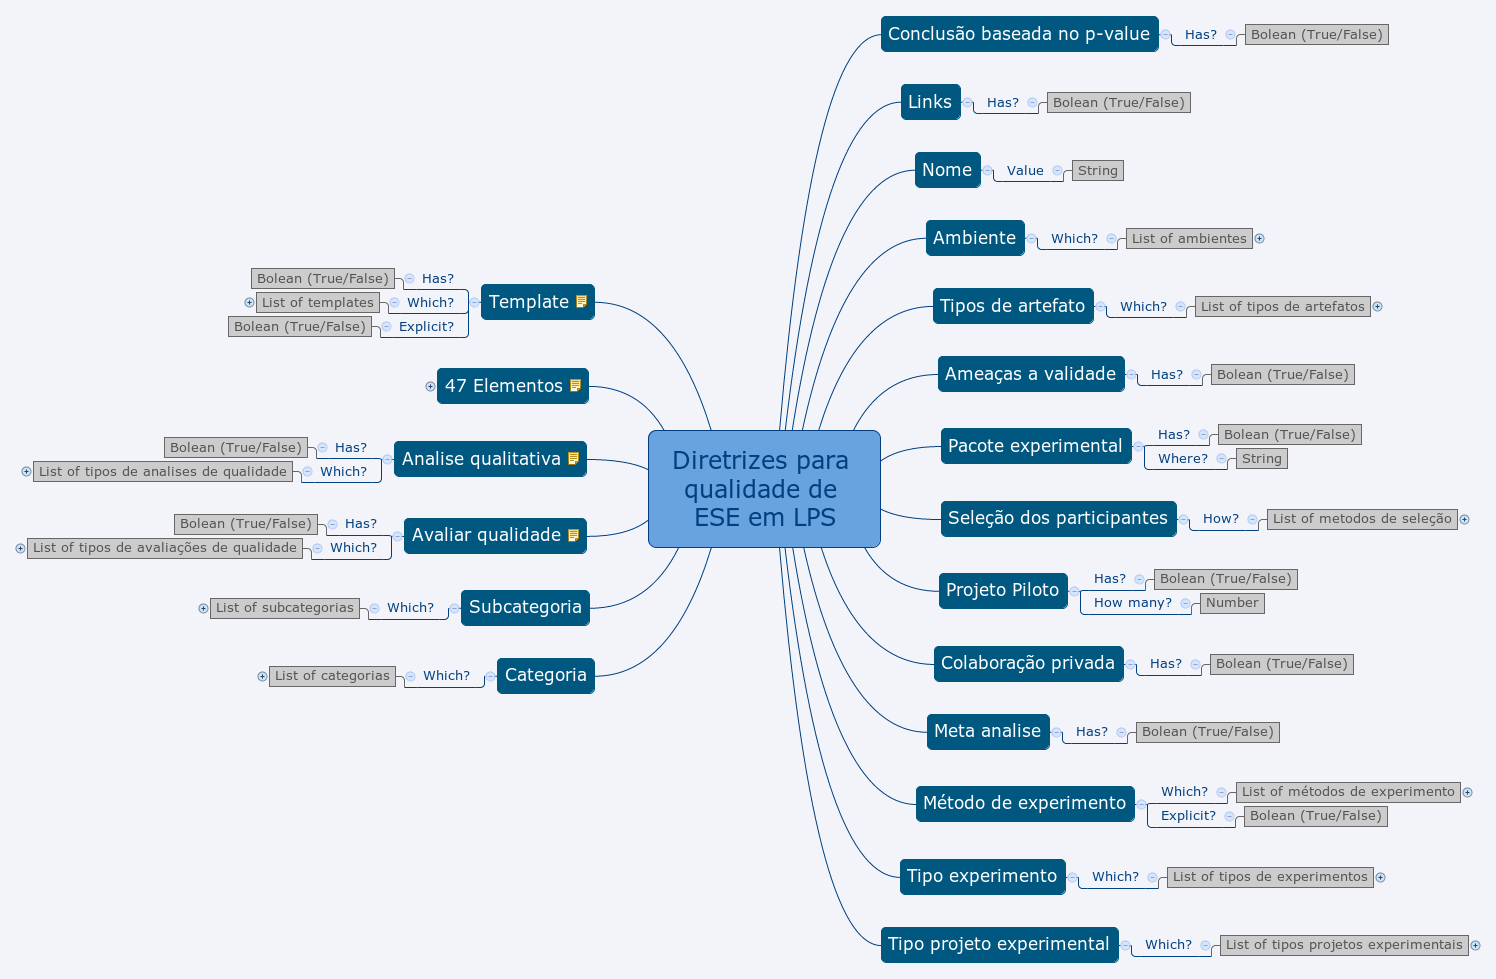
\includegraphics[scale=.3]{diretrizes_01.png}}
	
	\caption{Diretrizes da ontologia com mapa mental, classificação de domínios}
	\label{fig:diretrizes-01}
\end{figure}

\begin{figure}[h]
	\centering					
	{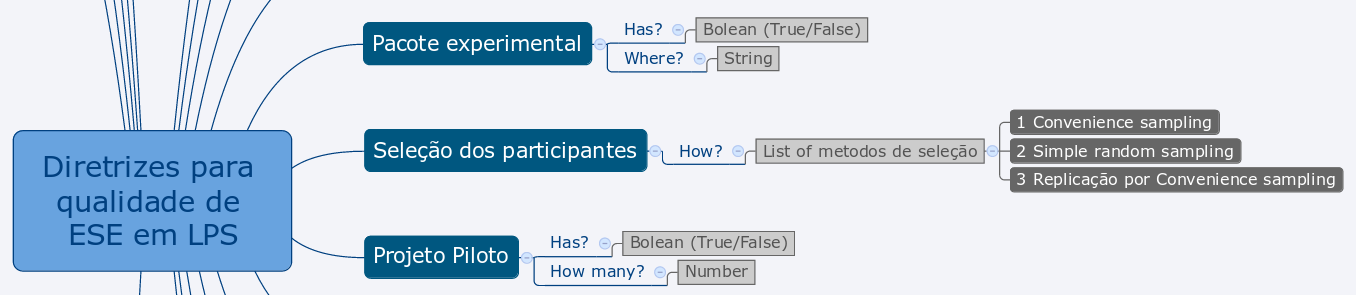
\includegraphics[scale=.3]{diretrizes_03.png}}
	
	\caption{Diretrizes da ontologia com mapa mental, exemplos de informações dos domínios classificados}
	\label{fig:diretrizes-03}
\end{figure}











